\chapter{单位、量纲与测量}\label{ch:b1:units-dimensions}

	在一间地下实验室里，单摆来回摆动，秒表咔嗒作响，
一名学生记下 $g = \qty{9.77}{m/s^2}$。这个值是“正确”的吗？
教材给出的是 $9.81$。两者是否相符，实验设计是否合理，
哪一步限制了实验的精度，这些都无法仅凭数字判断。
物理学是测量的科学，而没有不确定度的测量结果
只是一种传闻。本章将为此后各章建立共同的语言，
包括\omterm{def:b1:units-dimensions:unit}{单位}、\omterm{def:b1:units-dimensions:dimension}{量纲}、\omterm{def:b1:units-dimensions:oom}{数量级}，
以及不确定度的严谨运算。

\begin{omfigure}
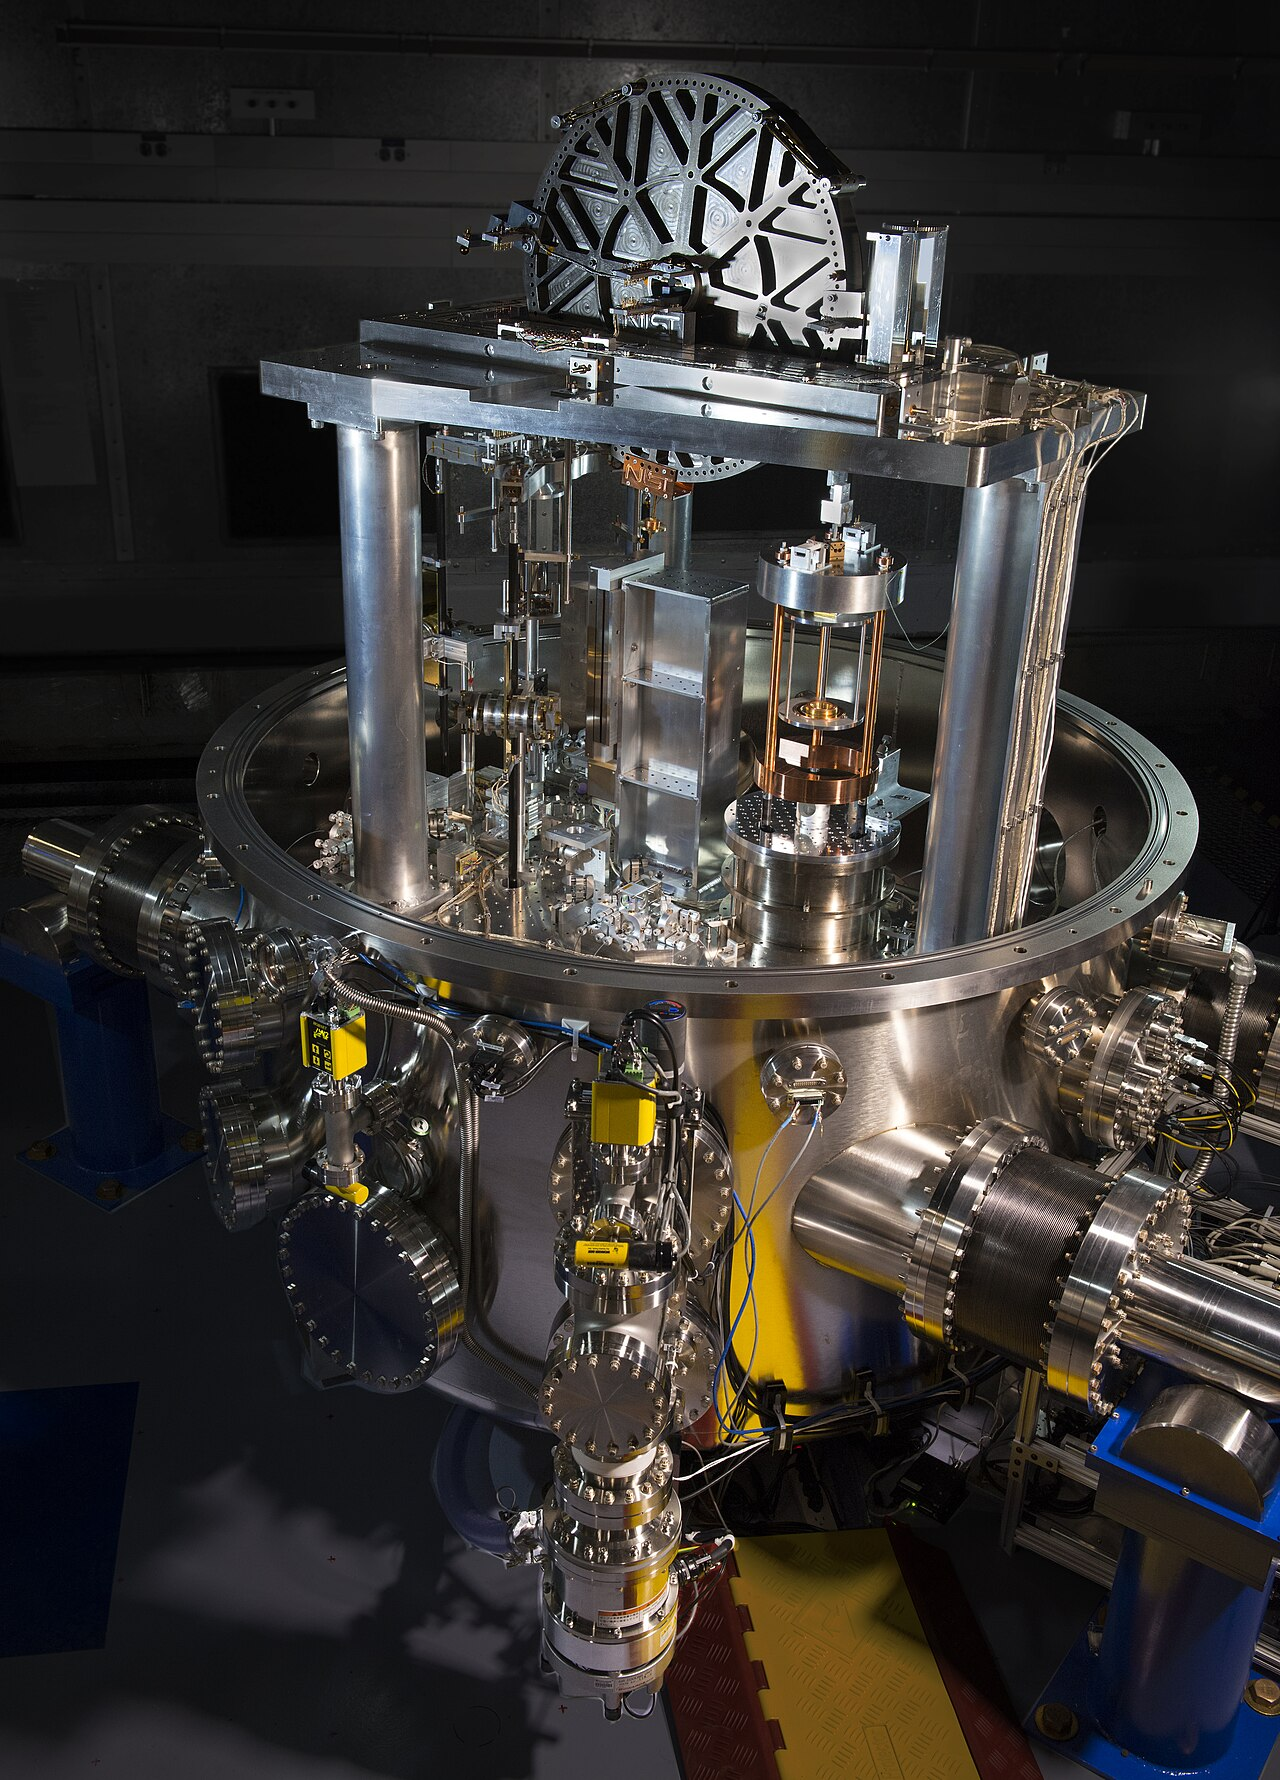
\includegraphics[width=0.46\linewidth]{images/book3/kibble-balance-nist.jpg}

{\small NIST-4 基布尔天平，是目前依据普朗克常量实现千克定义的仪器之一：质量与以电学\omterm{def:b1:units-dimensions:unit}{单位}测量的电磁力相平衡而被称量。照片：J.~L.~Lee，NIST（公有领域）。}
\end{omfigure}

\section{国际单位制}

\begin{definition}[物理量与单位]\label{def:b1:units-dimensions:unit}
称\emph{物理量}\index{物理量}为可以\omterm{def:b1:units-dimensions:uncertainty}{被测量}的一种性质，
例如长度、时长、质量和电流。测量某个物理量，
就是将它与同类的参考量相比较，这一参考量称为
\emph{单位}\index{单位}，测量结果等于一个数乘以单位，
如 $\ell = \qty{1.257}{m}$。仅有数字毫无意义，
仅有单位则测不出任何东西。
\end{definition}

\begin{definition}[国际单位制的基本单位]\label{def:b1:units-dimensions:si}
\index{国际单位制}\index{基本单位}
\emph{国际\omterm{def:b1:units-dimensions:unit}{单位}制}（SI）以七个
\emph{基本\omterm{def:b1:units-dimensions:unit}{单位}}：秒（\unit{s}）、米（\unit{m}）、
千克（\unit{kg}）、安培（\unit{A}）、开尔文（\unit{K}）、
摩尔（\unit{mol}）和坎德拉（\unit{cd}）。自 2019 年起，每个
基本\omterm{def:b1:units-dimensions:unit}{单位}都通过固定某一自然常数的数值来定义：
铯超精细跃迁频率 $\Delta\nu_{\mathrm{Cs}} = \qty{9192631770}{Hz}$
定义秒；光速 $c = \qty{299792458}{m/s}$ 则定义米；
普朗克常量
$h = \qty{6.62607015e-34}{J.s}$ 定义千克；元电荷
$e = \qty{1.602176634e-19}{C}$ 定义安培；玻尔兹曼常量
$k_B = \qty{1.380649e-23}{J/K}$ 定义开尔文；阿伏伽德罗常量
$N_A = \qty{6.02214076e23}{mol^{-1}}$ 定义摩尔；以及固定的发光效能
$K_{\mathrm{cd}}$ 定义坎德拉。其他每个\omterm{def:b1:units-dimensions:unit}{单位}都是
\emph{导出单位}\index{导出单位}，即基本\omterm{def:b1:units-dimensions:unit}{单位}的幂之积：
$\qty{1}{N} = \qty{1}{kg.m/s^2}$，$\qty{1}{J} = \qty{1}{N.m}$，
$\qty{1}{W} = \qty{1}{J/s}$，$\qty{1}{V} = \qty{1}{W/A}$，
$\qty{1}{Pa} = \qty{1}{N/m^2}$。
\end{definition}

\begin{omfigure}
\begin{tikzpicture}[font=\footnotesize, scale=0.95]
  \def\R{3.3} \def\r{1.75}
  \foreach \i/\a/\u/\c in {1/90/{\unit{s}}/{$\Delta\nu_{\mathrm{Cs}}$},
      2/141.4/{\unit{m}}/{$c$}, 3/192.9/{\unit{kg}}/{$h$},
      4/244.3/{\unit{A}}/{$e$}, 5/295.7/{\unit{K}}/{$k_B$},
      6/347.1/{\unit{mol}}/{$N_A$}, 7/38.6/{\unit{cd}}/{$K_{\mathrm{cd}}$}}{
    \node[draw, omDef, thick, circle, minimum size=8.2mm, fill=omDef!8]
      (U\i) at (\a:\R) {\u};
    \node[draw, omThm, circle, minimum size=7.5mm, fill=omThm!6]
      (C\i) at (\a:\r) {\c};
    \draw[-Stealth, omExo] (C\i) -- (U\i);
  }
  \draw[omExo, dashed, -Stealth] (U1) to[bend right=22] (U2);
  \draw[omExo, dashed, -Stealth] (U2) to[bend right=22] (U3);
  \draw[omExo, dashed, -Stealth] (U3) to[bend right=22] (U4);
\end{tikzpicture}

{\small 外环为七个\omterm{def:b1:units-dimensions:si}{基本单位}，内环为七个定义常数。固定常数只有
与已经定义的\omterm{def:b1:units-dimensions:unit}{单位}配合，才能定义对应的\omterm{def:b1:units-dimensions:unit}{单位}（虚线所示）：
$c$ 由秒定义米，$h$ 借助米和秒定义千克，
$e$ 借助秒
来定义安培。}
\end{omfigure}

\begin{remark}[名称与符号]\label{rem:b1:units-dimensions:names}
以人名命名的\omterm{def:b1:units-dimensions:unit}{单位}，全称用小写书写（牛顿、焦耳、
帕斯卡），符号则大写（\unit{N}、\unit{J}、\unit{Pa}）；
全称首字母大写时，该词即指那位科学家。词头按 10 的幂次递增，
由 p（$10^{-12}$）经 n、$\mu$、m、k、M、G 直至 T
（$10^{12}$）。
千克是名称中带有词头的唯一\omterm{def:b1:units-dimensions:si}{基本单位}。
\end{remark}

\begin{example}[拆解导出单位]\label{ex:b1:units-dimensions:unpack}
伏特：$\unit{V} = \unit{W/A} = \unit{J/(A.s)} = \unit{kg.m^2/(A.s^3)}$。
欧姆：$\unit{\ohm} = \unit{V/A} = \unit{kg.m^2/(A^2.s^3)}$。法拉：
$\unit{F} = \unit{C/V} = \unit{A.s/V} = \unit{A^2.s^4/(kg.m^2)}$。这类
拆解是检验公式是否被正确记住的最稳妥办法——
下一节将使这一做法系统化。
\end{example}

\section{量纲分析}

\begin{definition}[量纲]\label{def:b1:units-dimensions:dimension}
\index{量纲}\index{无量纲的}
\omterm{def:b1:units-dimensions:unit}{物理量} $X$ 的\emph{量纲}，记作 $[X]$，记录了 $X$
如何由七个基本量构成，与所选取的\omterm{def:b1:units-dimensions:unit}{单位}无关：
长度 $L$、质量 $M$、时间 $T$、电流 $I$、
温度 $\Theta$、物质的量 $N$、发光强度 $J$。
速率的量纲是 $[v] = L\,T^{-1}$，力的
量纲是 $[F] = M\,L\,T^{-2}$，能量的量纲是 $[E] = M\,L^2\,T^{-2}$。量纲为
$1$ 的量（如角度、比值、折射率）称为
\emph{无量纲的}。
\end{definition}

\begin{theorem}[量纲齐次性原理]\label{thm:b1:units-dimensions:homogeneity}
\index{量纲齐次性}
在物理定律中，等式两边具有相同的\omterm{def:b1:units-dimensions:dimension}{量纲}，
和式的每一项都与整体具有相同\omterm{def:b1:units-dimensions:dimension}{量纲}。指数函数、对数函数、正弦、余弦的
自变量是\omterm{def:b1:units-dimensions:dimension}{无量纲的}。
\end{theorem}

\begin{proof}
物理定律不依赖于人们选取的\omterm{def:b1:units-dimensions:unit}{单位}。将长度\omterm{def:b1:units-dimensions:unit}{单位}
改变为原来的 $\lambda$ 倍时，\omterm{def:b1:units-dimensions:dimension}{量纲}为
$L^a \cdots$ 的每个量都乘以 $\lambda^{-a}$：\omterm{def:b1:units-dimensions:dimension}{量纲}不同各项间的等式
在一种\omterm{def:b1:units-dimensions:unit}{单位}制中成立，在另一种中却不成立。
对于 $\exp$ 这类函数，级数
$1 + x + x^2/2 + \dots$ 会把不同\omterm{def:b1:units-dimensions:dimension}{量纲}的 $x$ 的幂相加，
除非 $x$ 是\omterm{def:b1:units-dimensions:dimension}{无量纲的}。
\end{proof}

\begin{method}[检验公式]\label{met:b1:units-dimensions:check}
\begin{enumerate}
  \item 写出每个符号的\omterm{def:b1:units-dimensions:dimension}{量纲}。
  \item 将每一边（每一项）化为乘积 $L^a M^b T^c \cdots$。
  \item 若两边指数相等，则公式\emph{可能}正确。
        若不相等，则公式必定错误：例如漏掉因子 $g$，
        本该是一次方的量写成了平方，
        或指数带有\omterm{def:b1:units-dimensions:dimension}{量纲}。
\end{enumerate}
\omterm{def:b1:units-dimensions:dimension}{量纲}齐次的公式仍可能相差一个无\omterm{def:b1:units-dimensions:dimension}{量纲}因子
（如 $2$、$\pi$、$\tfrac12$）：\omterm{def:b1:units-dimensions:dimension}{量纲}永远无法察觉这些因子。
\end{method}

\begin{example}[单摆的周期]\label{ex:b1:units-dimensions:pendulum}
长为 $\ell$、质量为 $m$ 的单摆在重力加速度 $g$ 下摆动。设
其周期为 $\tau = k\,\ell^\alpha m^\beta g^\gamma$，其中 $k$
于是 $T = L^\alpha M^\beta (L T^{-2})^\gamma =
L^{\alpha+\gamma} M^\beta T^{-2\gamma}$，故 $\beta = 0$，
$\gamma = -\tfrac12$，$\alpha = \tfrac12$：
\[
\tau = k\sqrt{\ell/g} .
\]
无需求解任何运动方程：质量消去，
长度加倍则周期变为原来的 $\sqrt2$ 倍。动力学
（见\cref{ch:b1:oscillators-resonance}）将给出
小幅摆动时的 $k = 2\pi$。
\end{example}

\begin{proposition}[无量纲组合]\label{prop:b1:units-dimensions:pi}
\index{无量纲组合}
若\omterm{def:b1:units-dimensions:unit}{物理量} $Y$ 依赖于 $n$ 个\omterm{def:b1:units-dimensions:unit}{物理量} $X_1, \dots, X_n$，它们
涉及 $r$ 个独立的基本\omterm{def:b1:units-dimensions:dimension}{量纲}，则该关系可改写为
$n + 1 - r$ 个由 $X_i$ 与 $Y$ 构成的\omterm{prop:b1:units-dimensions:pi}{无量纲组合}之间的关系。
当 $n + 1 - r = 1$ 时，唯一的组合必为常数，于是
\omterm{def:b1:units-dimensions:dimension}{量纲}分析可给出定律，至多差一个数值因子。
\end{proposition}
\admitted

\begin{remark}[命题的应用]\label{rem:b1:units-dimensions:pi}
一般表述（即瓦辛–白金汉定理）是
关于指数向量的一个线性代数问题。这里要紧的是方法：
列出相关的量，数出\omterm{def:b1:units-dimensions:dimension}{量纲}，构造\omterm{prop:b1:units-dimensions:pi}{无量纲组合}：
在\cref{ex:b1:units-dimensions:pendulum}中，$n = 3$
（$\ell, m, g$），$r = 3$（$L, M, T$），故存在唯一组合
$\tau\sqrt{g/\ell}$，它必为常数。半径为 $R$ 的球体
以速率 $v$ 运动，在密度为 $\rho$、黏度为 $\eta$ 的流体中，其阻力
涉及 $n = 4$ 个\omterm{def:b1:units-dimensions:unit}{物理量}与 $r = 3$ 个\omterm{def:b1:units-dimensions:dimension}{量纲}，共两个组合：
$F/(\rho v^2 R^2)$ 与 $\rho v R/\eta$（即雷诺数），
仅凭\omterm{def:b1:units-dimensions:dimension}{量纲}无法判断前者如何依赖后者——
这需要实验来确定。
\end{remark}

\section{数量级}

\begin{definition}[数量级]\label{def:b1:units-dimensions:oom}
\index{数量级}
\omterm{def:b1:units-dimensions:unit}{物理量}的\emph{数量级}是与之最接近的 10 的幂次：
$\qty{6.4e6}{m}$（地球半径）的数量级为
$10^7$；$\qty{3e3}{m}$ 的数量级为 $10^3$；$\qty{3.2e3}{m}$ 更接近
$10^3$ 而不是 $10^4$（在对数尺度上，分界点为
$\sqrt{10} \approx 3.16$）。两个量“同一数量级”是指
它们的比值小于约 $3$。
\end{definition}

\begin{method}[估算]\label{met:b1:units-dimensions:estimate}
对于一个无人测量过的量，估算方法如下：
\begin{enumerate}
  \item 将其分解为若干因子，每个因子的估计
        误差在 $2$ 或 $3$ 倍以内；
  \item 估计每个因子，保留一位\omterm{def:b1:units-dimensions:sigfig}{有效数字}；
  \item 相乘，保留 10 的幂次与一位数字。
\end{enumerate}
不同因子的误差部分相互抵消，结果通常在
$3$ 至 $10$ 倍之内是正确的，这往往已足以
判断一个假设成立与否。
\end{method}

\begin{example}[大气层的质量]\label{ex:b1:units-dimensions:atmosphere}
大气压强 $P_0 \approx \qty{1e5}{Pa}$，它是
一平方米上方空气柱的重力，$P_0 = m_{\text{气柱}}\,g$，故
$m_{\text{气柱}} \approx 10^5/10 = \qty{1e4}{kg}$（每平方米）。地球
表面积为 $4\pi R^2 \approx 4 \times 3 \times (6\times10^6)^2
\approx \qty{5e14}{m^2}$，大气层质量约为
$\qty{5e18}{kg}$。公认值为 $\qty{5.1e18}{kg}$——
估算只需要 $P_0$ 和 $R$。
\end{example}

\begin{definition}[有效数字]\label{def:b1:units-dimensions:sigfig}
\index{有效数字}
书写的数的\emph{有效数字}，是指从第一个非零
数字起的各位数字：$0.0820$ 有三位，$\num{8.20e-2}$ 同样有三位，
$820$ 有歧义（两位或三位），除非写成 \num{8.2e2} 或
\num{8.20e2}。结果应取其不确定度所允许的有效数字位数
（见下文\cref{met:b1:units-dimensions:writing}）：
而不应写成“$g = \qty{9.7723}{m/s^2}$”，当第四位数字未知时。
\end{definition}

\section{测量不确定度}

\begin{definition}[被测量、误差、不确定度]\label{def:b1:units-dimensions:uncertainty}
\index{被测量}\index{测量误差}\index{标准不确定度}
\emph{被测量}是指打算测量的量。重复
测量会得到分散的数值：测量是
\emph{可变的}。一次结果的\emph{误差}是其未知的
与真值之差；\emph{标准不确定度} $u(x)$ 为
结果 $x$ 的标准差，即人们可合理归于被测量的
各个取值的标准差——一个人们\emph{能够}
评估的量。其来源有：操作者（反应时间、视差）、
环境（温度、振动）、仪器（分辨率、
校准）、方法（仅近似成立的模型）。
\end{definition}

\begin{proposition}[A 类评定]\label{prop:b1:units-dimensions:typeA}
\index{不确定度!A 类}
由 $n$ 个独立重复值 $x_1, \dots, x_n$ 出发，
其均值 $\bar x = \frac1n \sum x_i$ 及实验标准差
\[
s = \sqrt{\frac{1}{n-1}\sum_{i=1}^n (x_i - \bar x)^2},
\]
则\omterm{def:b1:units-dimensions:uncertainty}{被测量}的最佳估计为 $\bar x$，其
\omterm{def:b1:units-dimensions:uncertainty}{标准不确定度}为
\[
u(\bar x) = \frac{s}{\sqrt n} .
\]
\end{proposition}

\begin{proof}[部分证明]
$s$ 估计单次测量的离散程度，这正是实验标准差的定义
（分母取 $n - 1$ 而非 $n$，因为
均值本身也由数据估计得到）。$n$ 个独立值之均值的
离散程度是单个值的 $\sqrt n$ 分之一，这源于
方差的可加性：$n$ 个独立变量之和的方差
是单个变量方差的 $n$ 倍，故均值的方差为
$s^2 n / n^2 = s^2/n$。这两个结论的严格证明
见本年度的概率课程。
\end{proof}

\begin{omfigure}
\begin{tikzpicture}
\begin{axis}[omaxis, width=9.6cm, height=5.6cm, xlabel={$T$ (\unit{s})},
    ylabel={次数}, ymin=0, ymax=16, xmin=1.962, xmax=2.058,
    xtick={1.97,1.99,2.01,2.03,2.05},
    x tick label style={/pgf/number format/fixed, /pgf/number format/precision=2}]
  \addplot[ybar, bar width=7.5pt, fill=omDef!35, draw=omDef] coordinates
    {(1.97,1) (1.98,3) (1.99,7) (2.00,12) (2.01,14) (2.02,8) (2.03,4) (2.04,1)};
  \addplot[omThm, thick, domain=1.962:2.058, samples=80] {12.5*exp(-((x-2.009)^2)/(2*0.016^2))};
  \draw[dashed, omExo] (axis cs:2.009,0) -- (axis cs:2.009,15.2) node[above, font=\footnotesize] {$\bar T$};
  \draw[Stealth-Stealth, omExo] (axis cs:1.993,7.6) -- (axis cs:2.025,7.6)
    node[midway, below, font=\footnotesize] {$2s$};
\end{axis}
\end{tikzpicture}

{\small 同一单摆周期的五十次计时，按
\qty{0.01}{s} 分组。其离散程度为 $s \approx \qty{0.016}{s}$（单次计时）；
五十次计时的均值之不确定度为 $s/\sqrt{50} \approx \qty{0.002}{s}$。
钟形曲线为具有相同均值与离散程度的高斯曲线。}
\end{omfigure}

\begin{proposition}[B 类评定]\label{prop:b1:units-dimensions:typeB}
\index{不确定度!B 类}
若某个值只读取一次，其不确定度依据
仪器已知的情况评定。若真值可在
$x - a$ 与 $x + a$ 之间任意取值且无偏好（即
半宽为 $a$ 的\emph{均匀}分布），
\[
u(x) = \frac{a}{\sqrt 3} .
\]
对于以步长 $\delta$ 刻划的刻度尺（半宽 $a = \delta/2$），
$u = \delta/(2\sqrt3) = \delta/\sqrt{12}$；数字显示器的
末位同样适用此式。制造商标注为
“$\pm a$”的公差，除非数据手册另有说明，
均按此方式处理。
\end{proposition}

\begin{proof}
在 $[x - a, x + a]$ 上均匀分布的方差为
$\frac{1}{2a}\int_{-a}^{a} t^2\,\dd t = \frac{1}{2a}\cdot\frac{2a^3}{3}
= \frac{a^2}{3}$；其标准差为 $a/\sqrt3$。
\end{proof}

\begin{omfigure}
\begin{tikzpicture}[font=\small, x=1.5cm, y=1.6cm]
  \draw[-Stealth] (-0.3,0) -- (4.3,0) node[right] {数值};
  \draw[-Stealth] (0,-0.15) -- (0,1.55) node[above] {密度};
  \draw[omDef, very thick] (0.3,0) -- (1.2,0) -- (1.2,1) -- (2.8,1) -- (2.8,0) -- (3.7,0);
  \fill[omDef!20] (1.2,0) rectangle (2.8,1);
  \node[below] at (1.2,0) {$x - a$};
  \node[below] at (2.8,0) {$x + a$};
  \node[below] at (2.0,0) {$x$};
  \node[left] at (0,1) {$\dfrac{1}{2a}$};
  \draw[dashed] (0,1) -- (1.2,1);
  \draw[Stealth-Stealth, omThm, thick] (2.0-0.577*0.8,1.18) -- (2.0+0.577*0.8,1.18)
    node[midway, above] {$2u = 2a/\sqrt3$};
  \draw[dashed, omThm] (2.0,0) -- (2.0,1.18);
\end{tikzpicture}

{\small 仅知读数位于 $\pm a$ 之内：均匀密度为
$1/(2a)$，标准差为 $a/\sqrt3 \approx 0.58\,a$——小于
$a$，因为两端的取值并不比中心更可能。}
\end{omfigure}

\begin{theorem}[合成不确定度]\label{thm:b1:units-dimensions:propagation}
\index{不确定度!合成}\index{不确定度的传播}
设 $y = f(x_1, \dots, x_n)$ 由独立测量值计算得出，
各测量值的\omterm{def:b1:units-dimensions:uncertainty}{标准不确定度}为 $u(x_i)$。则
\[
u(y)^2 = \sum_{i=1}^n \left(\frac{\partial f}{\partial x_i}\right)^2 u(x_i)^2 .
\]
特别地：
\begin{itemize}
  \item 和或差 $y = x_1 \pm x_2$：
        $u(y)^2 = u(x_1)^2 + u(x_2)^2$；
  \item 积或商 $y = x_1 x_2$ 或 $x_1/x_2$：
        $\left(\dfrac{u(y)}{y}\right)^2 = \left(\dfrac{u(x_1)}{x_1}\right)^2
        + \left(\dfrac{u(x_2)}{x_2}\right)^2$；
  \item 幂次 $y = k\,x^\alpha$：$\dfrac{u(y)}{\abs y} = \abs\alpha\,\dfrac{u(x)}{\abs x}$。
\end{itemize}
\end{theorem}

\begin{proof}
对于小偏差 $\delta x_i$，一阶泰勒展开
给出 $\delta y = \sum_i (\partial f/\partial x_i)\,\delta x_i$。各偏差
相互独立且均值为零，故和的方差
等于各方差之和，每项乘以其系数的平方
——即上式。特殊情形由此得出：
$\partial(x_1 x_2)/\partial x_1 = x_2$，故
$u(y)^2 = x_2^2 u(x_1)^2 + x_1^2 u(x_2)^2$，两边除以 $y^2 = x_1^2 x_2^2$；
对于 $y = kx^\alpha$，$\partial y/\partial x = \alpha y/x$。
\end{proof}

\begin{example}[圆柱体的密度]\label{ex:b1:units-dimensions:density}
圆柱体：$m = \qty{47.32}{g}$（$u = \qty{0.01}{g}$），
$d = \qty{12.00}{mm}$（$u = \qty{0.02}{mm}$），$h = \qty{50.2}{mm}$
（$u = \qty{0.1}{mm}$）。$\rho = 4m/(\pi d^2 h)$，故相对
不确定度的平方相加为 $(0.01/47.32)^2 = \num{4.5e-8}$，
$(2 \times 0.02/12.00)^2 = \num{1.1e-5}$ 与
$(0.1/50.2)^2 = \num{4.0e-6}$ 之和：直径占主导，因为它
被平方，且测量精度为 $0.17\%$。$u(\rho)/\rho = \sqrt{\num{1.5e-5}}
= 0.39\%$；$\rho = \qty{8334}{kg/m^3}$，故 $u(\rho) = \qty{33}{kg/m^3}$：
$\rho = (8.33 \pm 0.03)\times10^3\ \unit{kg/m^3}$——黄铜。
\end{example}

\begin{method}[写出结果]\label{met:b1:units-dimensions:writing}
\begin{enumerate}
  \item 将不确定度修约为一位\omterm{def:b1:units-dimensions:sigfig}{有效数字}（若首位数字
        为 $1$ 或 $2$ 时取两位）。
  \item 将测量值修约到相同的小数位。
  \item 写出数值及不确定度，并附\omterm{def:b1:units-dimensions:unit}{单位}：
        $g = \qty{9.77\pm0.03}{m/s^2}$，或 $g = \qty{9.77}{m/s^2}$，
        $u(g) = \qty{0.03}{m/s^2}$。
\end{enumerate}
\emph{计算过程中}应保留多余位数，只在最后才修约。
\end{method}

\begin{definition}[归一化偏差]\label{def:b1:units-dimensions:zscore}
\index{归一化偏差}\index{两个结果的相容性}
同一\omterm{def:b1:units-dimensions:uncertainty}{被测量}的两个结果 $x_1 \pm u_1$ 与 $x_2 \pm u_2$ 通过
它们的\emph{归一化偏差}进行比较：
\[
z = \frac{\abs{x_1 - x_2}}{\sqrt{u_1^2 + u_2^2}} .
\]
当 $z \leq 2$ 时二者\emph{相容}；$z$ 较大则说明存在
未计入的效应——或不确定度被低估。若 $x_2$ 为
没有给出不确定度的参考值，则取 $u_2 = 0$。
\end{definition}

\begin{remark}[为何取 2]\label{rem:b1:units-dimensions:why2}
若两个结果服从高斯分布，则它们之差的标准差
为 $\sqrt{u_1^2 + u_2^2}$，高斯变量超出其两倍标准差的
情形约占 $5\%$。“$z \leq 2$”是一种
约定，而非定理：它会把大约每二十次良好测量中的一次
误判为虚假的不一致。
\end{remark}

\section{用数据拟合模型}

\begin{proposition}[最小二乘直线]\label{prop:b1:units-dimensions:regression}
\index{线性回归}\index{最小二乘法}
设 $n$ 个点 $(x_i, y_i)$ 应满足 $y = a x + b$，则使
竖直距离的平方和
$\sum_i (y_i - a x_i - b)^2$ 最小的直线为
\[
a = \frac{\sum_i (x_i - \bar x)(y_i - \bar y)}{\sum_i (x_i - \bar x)^2},
\qquad
b = \bar y - a\,\bar x .
\]
\end{proposition}

\begin{proof}
上式是关于 $(a, b)$ 的二次函数，令两个偏导数
均为零，得两个线性方程：$\sum_i (y_i - ax_i - b) = 0$，
即 $\bar y = a \bar x + b$，以及 $\sum_i x_i (y_i - ax_i - b) = 0$。
将 $b$ 代入第二式并对变量作中心化，即得 $a$。
极小化的具体过程在数学课程中
关于二元函数的部分给出。
\end{proof}

\begin{method}[用图像检验模型]\label{met:b1:units-dimensions:fit}
\begin{enumerate}
  \item 选取使预期规律成为直线的变量：
        单摆取 $\tau^2$ 对 $\ell$，对幂律取 $\ln y$ 对
        $\ln x$，即 $y = Cx^\alpha$（斜率为 $\alpha$）。
  \item 描出数据点，\emph{并附上不确定度棒}。
  \item 拟合直线；若不确定度棒穿过直线，
        残差无系统性趋势，且截距与模型预测相符
        （此处为零），则模型可接受。
  \item 由斜率及其不确定度读取物理结果。
\end{enumerate}
\end{method}

\begin{omfigure}
\begin{tikzpicture}
\begin{axis}[omaxis, width=9.4cm, height=6cm, xlabel={$\ell$ (\unit{m})},
    ylabel={$\tau^2$ (\unit{s^2})}, xmin=0, xmax=1.35, ymin=0, ymax=5.4,
    xtick={0,0.4,0.8,1.2}, ytick={0,1,2,3,4,5}]
  \addplot[omThm, thick, domain=0:1.3, samples=2] {4.035*x + 0.004};
  \addplot[only marks, mark=*, omDef, error bars/.cd, y dir=both, y explicit]
    coordinates {(0.400,1.62) +- (0,0.02) (0.600,2.41) +- (0,0.02)
                 (0.800,3.25) +- (0,0.03) (1.000,4.04) +- (0,0.04)
                 (1.200,4.84) +- (0,0.05)};
\end{axis}
\end{tikzpicture}

{\small 五个单摆摆长下的 $\tau^2$ 对 $\ell$ 关系，带
不确定度棒；最小二乘直线在不确定度范围内过原点，
其斜率 $4\pi^2/g$ 给出 $g$。}
\end{omfigure}

\begin{example}[由斜率读取 $g$]\label{ex:b1:units-dimensions:slope}
图中五个数据点的 $\bar\ell = \qty{0.800}{m}$，
$\overline{\tau^2} = \qty{3.232}{s^2}$，两个和分别为
$\sum (\ell_i - \bar\ell)(\tau_i^2 - \overline{\tau^2}) = \qty{1.614}{m.s^2}$，
$\sum (\ell_i - \bar\ell)^2 = \qty{0.400}{m^2}$：斜率
$a = \qty{4.035}{s^2/m}$，截距 $b = \qty{0.004}{s^2}$，可忽略。由
$\tau^2 = (4\pi^2/g)\,\ell$，故 $g = 4\pi^2/a = \qty{9.78}{m/s^2}$。
\end{example}

\section{练习}

\begin{exercise}[$\star$]\label{exo:b1:units-dimensions:1}
用\omterm{def:b1:units-dimensions:si}{基本单位}表示焦耳、瓦特、帕斯卡和库仑。
由此推断 $\unit{Pa.m^3}$ 是能量的\omterm{def:b1:units-dimensions:unit}{单位}。
\end{exercise}

\begin{exercise}[$\star$]\label{exo:b1:units-dimensions:2}
求压强、功率、电荷和电压的\omterm{def:b1:units-dimensions:dimension}{量纲}，以及
常量 $G$（在 $F = Gm_1m_2/r^2$ 中）、$h$（在
$E = h\nu$ 中）和 $k_B$（在 $E = k_B T$ 中）的\omterm{def:b1:units-dimensions:dimension}{量纲}。
\end{exercise}

\begin{exercise}[$\star$]\label{exo:b1:units-dimensions:3}
这些公式是否\omterm{def:b1:units-dimensions:dimension}{量纲}齐次？$v = \sqrt{2gh}$；
$E = \tfrac12 m v$；$P = \rho g h$ 表示压强；$x = v_0 t +
\tfrac12 g t^2$；$T = 2\pi\sqrt{g/\ell}$；$I = I_0 \eu^{-t/RC}$。
\end{exercise}

\begin{exercise}[$\star$]\label{exo:b1:units-dimensions:4}
刻度尺以毫米分度；电子天平的显示步长为
\qty{0.01}{g}；电压表的说明书保证“$\pm 0.5\%$ 的
读数”。求 \qty{12.7}{cm} 长度、
\qty{5.43}{g} 质量及 \qty{4.80}{V} 读数的 B 类\omterm{def:b1:units-dimensions:uncertainty}{标准不确定度}。
\end{exercise}

\begin{exercise}[$\star\star$]\label{exo:b1:units-dimensions:5}
绷紧弦上波的速率 $v$ 取决于其张力 $F$
（一种力）和其线密度 $\mu$。求 $v$ 的表达式，
允许相差一个无\omterm{def:b1:units-dimensions:dimension}{量纲}因子。对压强为 $P$、密度为
$\rho$ 的气体中的声速，求解同样的问题。
\end{exercise}

\begin{exercise}[$\star\star$]\label{exo:b1:units-dimensions:6}
同一次下落的八次计时（\omterm{def:b1:units-dimensions:unit}{单位}为毫秒）：$452$、$447$、$461$、
$455$、$449$、$458$、$444$、$454$。计算平均值、实验标准差
及平均值的\omterm{def:b1:units-dimensions:uncertainty}{标准不确定度}；
写出结果。
\end{exercise}

\begin{exercise}[$\star\star$]\label{exo:b1:units-dimensions:7}
某电阻按 $R = U/I$ 测量，其中 $U = \qty{4.80}{V}$，
$u(U) = \qty{0.03}{V}$，$I = \qty{12.4}{mA}$，$u(I) = \qty{0.2}{mA}$。
计算 $R$ 和 $u(R)$；哪一个测量应首先改进？
\end{exercise}

\begin{exercise}[$\star\star$]\label{exo:b1:units-dimensions:8}
两个小组测量声速，分别得到 $\qty{343\pm4}{m/s}$ 和
$\qty{336\pm3}{m/s}$。它们是否相容？第三个小组得到
$\qty{352\pm2}{m/s}$：与第一组相容吗？与第二组呢？
\end{exercise}

\begin{exercise}[$\star\star$]\label{exo:b1:units-dimensions:9}
球体的体积由其直径 $d = \qty{25.40}{mm}$ 算出，
直径用游标卡尺测量，$u(d) = \qty{0.02}{mm}$。计算 $V$，
其相对不确定度和绝对不确定度，并写出结果。
\end{exercise}

\begin{exercise}[$\star\star\star$]\label{exo:b1:units-dimensions:10}
半径为 $R$ 的小球在黏性液体中缓慢下落，阻力
取决于 $R$、速率 $v$ 和黏度 $\eta$，后者的\omterm{def:b1:units-dimensions:dimension}{量纲}为 $M L^{-1} T^{-1}$。证明 $F = k\,\eta R v$。
在高速时，
阻力改为取决于 $R$、$v$ 和流体密度 $\rho$：
求出新的规律。对雨滴（$R = \qty{1}{mm}$，
$v = \qty{5}{m/s}$，空气：$\rho = \qty{1.2}{kg/m^3}$，
$\eta = \qty{1.8e-5}{Pa.s}$）作估算，通过比较两个
估计值判断哪一种情形适用。
\end{exercise}

\begin{exercise}[$\star\star\star$]\label{exo:b1:units-dimensions:11}
对电阻两端的电压进行四次测量，电流依次增大：
$(I, U) = (\qty{2.0}{mA}, \qty{0.41}{V})$，$(\qty{4.0}{mA},
\qty{0.78}{V})$，$(\qty{6.0}{mA}, \qty{1.22}{V})$，$(\qty{8.0}{mA},
\qty{1.59}{V})$。计算最小二乘斜率与截距，由此求得
$R$；若每个 $U$ 的不确定度均为
$u = \qty{0.02}{V}$，截距是否与零相容？
\end{exercise}

\begin{exercise}[$\star\star\star$]\label{exo:b1:units-dimensions:12}
由 $G = \qty{6.67e-11}{m^3/(kg.s^2)}$、$h = \qty{6.63e-34}{J.s}$ 和
$c = \qty{3.00e8}{m/s}$，由\omterm{def:b1:units-dimensions:dimension}{量纲}分析构造一个长度、一个
时间与质量（即普朗克\omterm{def:b1:units-dimensions:unit}{单位}）。计算它们，并与
质子的尺度（\qty{1e-15}{m}）及人的质量相比较。
\end{exercise}

\begin{omfigure}
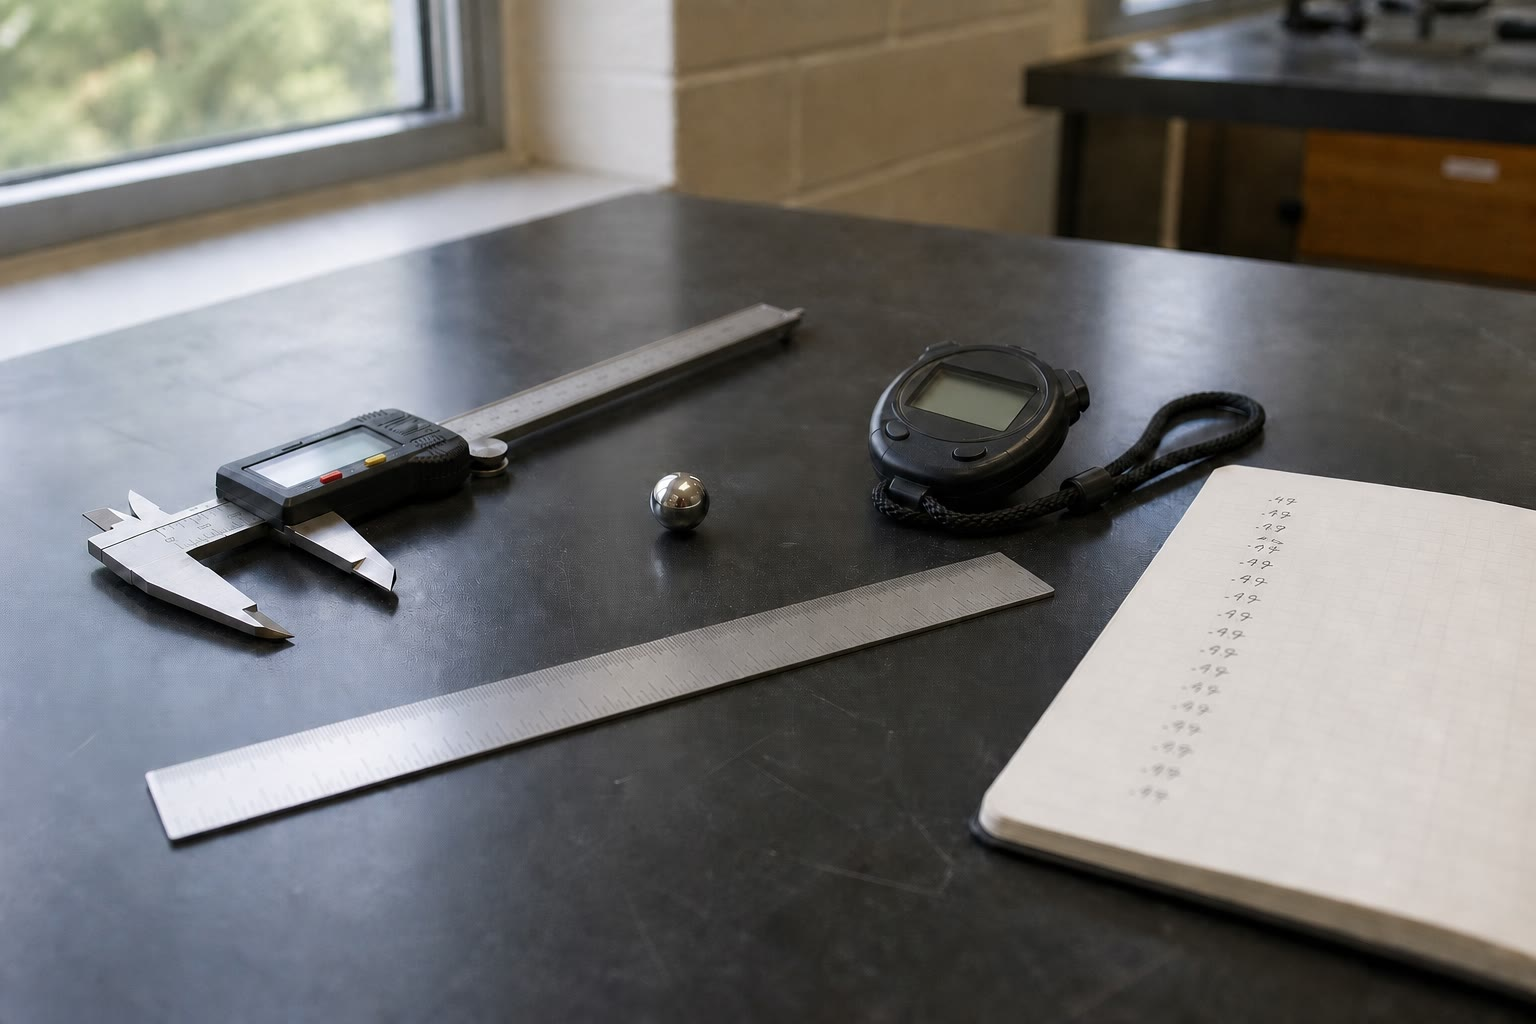
\includegraphics[width=0.60\linewidth]{images/book3/ai/b3-01-lab-bench-measuring.jpg}

{\small 本章的原材料：游标卡尺、秒表、小球、直尺，以及一列彼此总不完全一致的重复读数。}
\end{omfigure}

\section{问题：用单摆测量 $g$}

\begin{problem}[{周末问题——一根细线、一个摆球、一只秒表和一把
卷尺：一张厨房餐桌能以多高精度测量地球的引力场，
以及其四个数中哪一个是薄弱环节}]
\label{pb:b1:units-dimensions:1}
单摆是用一根轻绳悬挂于固定点的钢球；
小角度摆动的周期为 $\tau = 2\pi\sqrt{\ell/g}$，其中 $\ell$ 为
悬挂点到摆球球心的距离。本题的目标是得到一个
具有可靠不确定度的 $g$ 值。

\medskip
\noindent\textbf{第一部分——模型。}
\begin{enumerate}
  \item 检验 $\tau = 2\pi\sqrt{\ell/g}$ 的\omterm{thm:b1:units-dimensions:homogeneity}{量纲齐次性}。
  \item 小球的质量为 $m$。仅由\omterm{def:b1:units-dimensions:dimension}{量纲}论证，周期
        不可能依赖于 $m$：若它仅依赖于 $\ell$、$g$
        和 $m$。
  \item 周期还会略微依赖于摆动的振幅 $\theta_0$，
        \omterm{def:b1:units-dimensions:dimension}{量纲}分析为何允许这种依赖？实验上
        必须怎样做才能使公式适用？
  \item 将 $g$ 表示为 $\ell$ 和 $\tau$ 的函数。
\end{enumerate}

\medskip
\noindent\textbf{第二部分——测量长度。}
卷尺以毫米为分度；细线
从悬挂点到摆球顶端的长度为 \qty{99.0}{cm}，摆球的
直径为 \qty{2.00}{cm}，两者均只读取一次。
\begin{enumerate}[resume]
  \item 计算 $\ell$。
  \item 估计卷尺上单次读数的
        B 类不确定度。
  \item 确定悬挂点与摆球球心的位置会额外引入
        估计可能误差为 $\pm\qty{5}{mm}$（均匀分布）。将其与
        上一小题合成为 $u(\ell)$，并给出相对不确定度
        $u(\ell)/\ell$。
\end{enumerate}

\medskip
\noindent\textbf{第三部分——测量周期。}
为减小反应时间的影响，每次计时十个周期。共做
八次计时（\omterm{def:b1:units-dimensions:unit}{单位}：秒）依次为 $20.12$、$20.05$、$20.18$、$20.09$、$20.15$、
$20.02$、$20.11$、$20.08$。
\begin{enumerate}[resume]
  \item 为何计时十个周期而不是一个？为何要重复
        计时八次？
  \item 计算八次计时的平均值 $\overline{t_{10}}$ 与实验
        标准差 $s$。
  \item 推出平均值的\omterm{def:b1:units-dimensions:uncertainty}{标准不确定度}，进而求出周期
        $\tau$ 及其不确定度 $u(\tau)$。
  \item 比较 $u(\tau)/\tau$ 与 $u(\ell)/\ell$。
\end{enumerate}

\medskip
\noindent\textbf{第四部分——结果及其薄弱环节。}
\begin{enumerate}[resume]
  \item 计算 $g$。
  \item 将 $u(g)/g$ 用 $u(\ell)/\ell$ 与 $u(\tau)/\tau$ 表示，
        并计算其数值。
  \item 将结果写成标准形式。
  \item 通过\omterm{def:b1:units-dimensions:zscore}{归一化偏差}，将结果与参考值 $\qty{9.81}{m/s^2}$ 比较，
        结论如何？
  \item 两个\omterm{def:b1:units-dimensions:uncertainty}{被测量}中哪一个限制了
        $g$ 的精度？提出两项具体改进，并说明各自
        能将相对不确定度降低多少。
  \item 假设由于对齐不仔细，每个长度都被
        高估了 \qty{5}{mm}。这一误差是否已计入
        不确定度预算？这类误差叫什么名称，
        又该如何发现？
\end{enumerate}

\medskip
\noindent\textbf{第五部分——五个长度与一条直线。}
重复实验，分别取 $\ell = 0.400$、$0.600$、$0.800$、
$1.000$ 和 \qty{1.200}{m}，得到 $\tau^2 = 1.62$、$2.41$、$3.25$、
$4.04$ 和 \qty{4.84}{s^2}，其不确定度均约为 $u(\tau^2) \approx 1\%$。
\begin{enumerate}[resume]
  \item 为何以 $\tau^2$ 对 $\ell$ 作图，
        而不以 $\tau$ 对 $\ell$ 作图？
  \item 计算 $\bar\ell$ 与 $\overline{\tau^2}$。
  \item 计算最小二乘斜率 $a$ 与截距 $b$。
  \item 由斜率推出 $g$。
  \item 解释截距的含义：若 $b$ 明显不为零，
        将揭示什么？
  \item 计算机拟合给出 $u(a) = \qty{0.05}{s^2/m}$。由此推出
        $u(g)$ 并写出结果。
  \item 用\omterm{def:b1:units-dimensions:zscore}{归一化偏差}比较第四部分的单一长度结果
        与本部分的结果。
  \item 有学生提议，改用同一卷尺与秒表，在楼梯井里
        测量一个 \qty{10}{m} 长的单摆的一次摆动，
        估计由此得到的 $g$ 的相对不确定度，
        并就最佳策略作出结论。
\end{enumerate}
\end{problem}
